\documentclass[dissertation.tex]{subfiles}

\begin{document}

% Start here (11/05/2019)
% Don't let Andrius distract...

\section{Success Criteria}
{
    The success criteria laid out in the project proposal have all been satisfied:

    \begin{itemize}
    \item Translate simple Haskell programs into executable Java bytecode.
    \item Reject ill-formed programs due to syntactic or type errors.
    \item Perform simple optimisations during translation.
    \item Perform evaluation using non-strict semantics.
    \end{itemize}
    
    Beyond these base requirements, a number of the extensions implementing language features have been completed
    successfully.

    \todo[inline]{Mention somewhere pros/cons of using JVB}
}
\section{Language Features}
{
    The planned subset of Haskell encompassed functions, arithmetic, booleans, lists, simple typeclasses, and laziness. The following program is compilable using my compiler (it is even included as a test), and demonstrates various use-cases of all of these features:

    \begin{haskellfigure}
    -- foldl :: (b -> a -> b) -> b -> [a] -> b
    foldl _ e [] = e
    foldl f e (x:xs) = foldl f (f e x) xs

    -- sum :: Num a => [a] -> a
    sum = foldl (+) 0

    -- take :: Int -> [a] -> [a]
    take 0 _ = []
    take _ [] = undefined
    take n (x:xs) = x:take (n-1) xs

    -- ones :: Num a => [a]
    ones = 1:ones

    -- valid :: Bool
    valid = sum (take 10 ones :: [Int]) == 10
    \end{haskellfigure}

    \todo[inline]{Make a bigger deal out of the working bits? More demonstrations of laziness etc?}

    Successfully implemented extensions include support for user-defined datatypes, user-defined typeclasses and instances, monads, and some syntactic features like operator sections and support for point-free notation: these can be demonstrated by the following program:

    \todo[inline]{Hard to give an example program using monads without ending up doing a monad tutorial!}
    \begin{haskellfigure}
    data Maybe a = Nothing | Just a
    data [] a = [] | a:[a]
    
    class Monad m where
        (>>=) :: m a -> (a -> m b) -> m b
        return :: a -> m a
    instance Monad Maybe where
        Nothing >>= f = Nothing
        (Just x) >>= f = f x
        return = Just
    instance Monad [] where
        [] >>= f = []
        (x:xs) >>= f = (f x) ++ (f >>= xs)
        return x = [x]

    -- The monad instance for maybe can be interpreted as function application
    -- with support for chaining failure
    divide x y = if y == 0 then Nothing else Just (x / y)
    x = divide 4 0 >>= divide 20 -- Evaluates to Nothing

    -- The monad instance for lists can be interpreted as performing
    -- non-deterministic computation: each step can have multiple results
    countdown 0 = []
    countdown n = n:countdown (n - 1)
    onlyEven x = if even x then [x] else []
    y = [1,2,3] >>= countdown -- Evaluates to [1,2,1,3,2,1]
    z = y >>= onlyEven -- Evaluates to [2,2]
    \end{haskellfigure}

    Each simple feature name necessarily glosses over many smaller constituent features necessary for use. For example, the `lists' feature allows for lists to be created using either the plain constructor syntax (\haskell{1:(2:(3:[]))}) or syntactic sugar for lists (\haskell{[1,2,3]}), and matched using patterns (eg.\ \haskell{[x,y] = [1,2]}). However, there's no support for list comprehensions (eg.\ \haskell{[f x | x <- [1,2,3], even x]}) as they weren't a high priority feature.
    
    \subsubsection{Correctness}
    {
        Correctness of the various stages of the compiler has been empirically tested using a large set of unit, integration, and regression tests: these include tests of complete programs, such as those used for benchmarking.
        
        At the time of writing, there are 245 tests. These are run both on my development machine (described in Section \ref{sec:test-environment}), and on machines provided by Travis CI\footnote{\url{https://travis-ci.org/hnefatl/dissertation-project}} whenever a commit is pushed to my development GitHub repository. This ensures the compiler works in a clean, reproducible environment and not just on my development system.

        Bugs found and fixed during development have at least one associated regression test to ensure that they cannot reappear.

        As the compiler is developed using Haskell, some forms of compiler bugs that could affect the correctness of translation have been mitigated: type errors and bugs due to mutable state cannot exist within the compiler.
    }
}
\section{Performance}
{
    Although performance was not an important aspect of the success criteria, it's still interesting to evaluate the effectiveness of optimisations on the output program, and the performance of the compiler and its output compared to other Haskell to JVB compilers.

    The two compilers used for comparisons are Eta and Frege. Eta is a fork of GHC that replaces the backend with one targeting JVB: it can take advantage of the powerful optimisations already available in the front- and middle-end of GHC, which is the world-leading Haskell compiler, so I expected it to perform better than both my compiler and Frege. Frege is a from-scratch compiler that compiles to Java instead of JVB, then uses a Java compiler to produce JVB. I expect Frege to perform better than my compiler, given the maturity of the project (under development since at least 2011).

    Both Eta and Frege enable optimisations by default, so all metrics given for them have optimisations enabled. Metrics given for my compiler are labelled to indicate whether or not optimisations have been applied.

    \subsection{Test Environment}\label{sec:test-environment}
    {
        Benchmarks were performed as the only active process on my development machine: a ThinkPad 13 running Debian 9 with 8GB RAM and an Intel Core i5-7200U CPU (2.5GHz).
    }
    \subsection{Benchmark Approach}
    {
        All of the compilers being compared output JVB, so a natural choice of benchmarking framework was the Java Microbenchmark Harness (JMH)\footnote{\url{https://openjdk.java.net/projects/code-tools/jmh/}}. This allows for accurate Java program benchmarking by handling JVM warmup, disabling garbage collection, etc. There are downsides to the framework though, notably that it doesn't record memory usage, and that it only appears to expose percentiles and histograms of the results through its Java API, not the raw data.

        To measure compiler performance, a more na{\"i}ve approach was taken: the execution times of 50 sequential compilations were recorded for each compiler.
        
        For my compiler, the time taken to write the compiled class files to disk and compress them into a jar file was computed by measuring the difference between compilation runs which write to disk, and those which don't (using the \monospace{--no-write-jar} command-line-flag). This data is used in Figure \ref{fig:compiler-perf}.
    }
    \subsection{Execution Speed}
    {
        Figure \ref{fig:perf} demonstrates the runtime performance of the benchmark programs after compilation by the different compilers. It is evident that the performance of programs compiled by my compiler is significantly lower than those from Frege or Eta, but also that applying optimisations can produce a reasonable speedup.

        Interestingly Frege produced more performant programs than Eta, which wasn't expected, given that Eta leverages the work done on the GHC compiler.

        \begin{figure}[h]
            \centering
            \captionsetup{width=0.8\textwidth}
            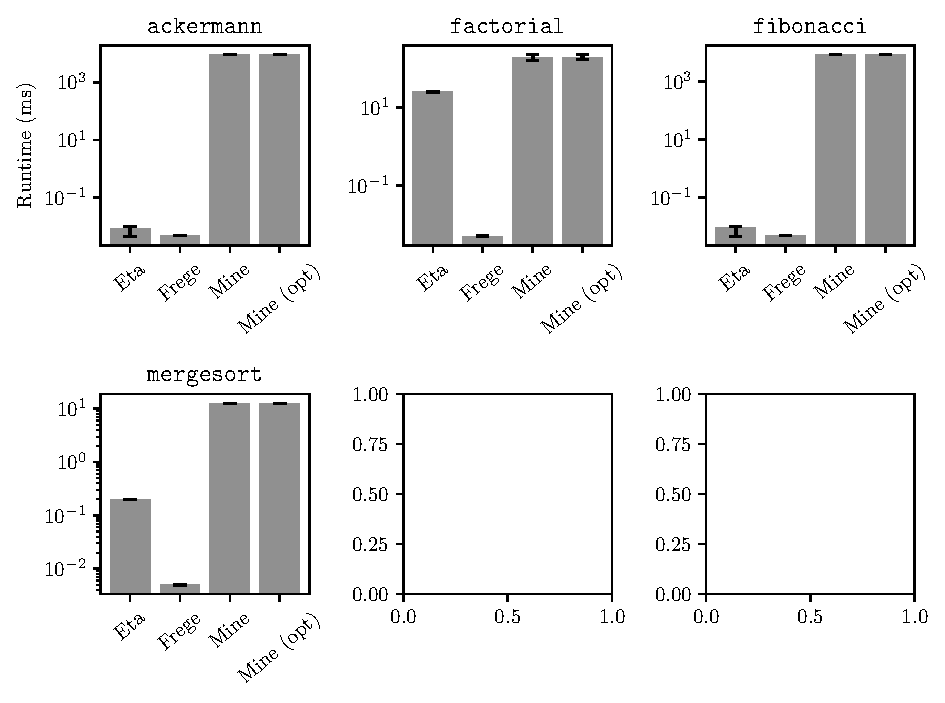
\includegraphics[width=0.9\textwidth]{graphs/perf.pdf}
            \caption{Median runtime in milliseconds of the benchmark programs. Error bars show 25th and 75th percentiles.}
            \label{fig:perf}

            \todo[inline]{Update to use min with error bars showing 25th+50th quartile or similar}
        \end{figure}

        The inefficiency of programs output by my compiler seems to stem primarily from my implementation of runtime closures (described in Section \ref{sec:closures}). Figure \ref{fig:inner-time} shows that almost 40\% of a program's execution is spent in the functions associated with creating and calling closures: \monospace{enter}, \monospace{addArgument}, and \monospace{clone}. A more efficient implementation should have most of the runtime spent in one or more of the \monospace{Impl} functions (such as \monospace{_v19Impl}), which perform the actual logic of an expression of the Haskell program, rather than the bottleneck being in the runtime system.

        \begin{figure}[h]
            \centering
            \captionsetup{width=0.9\textwidth}
            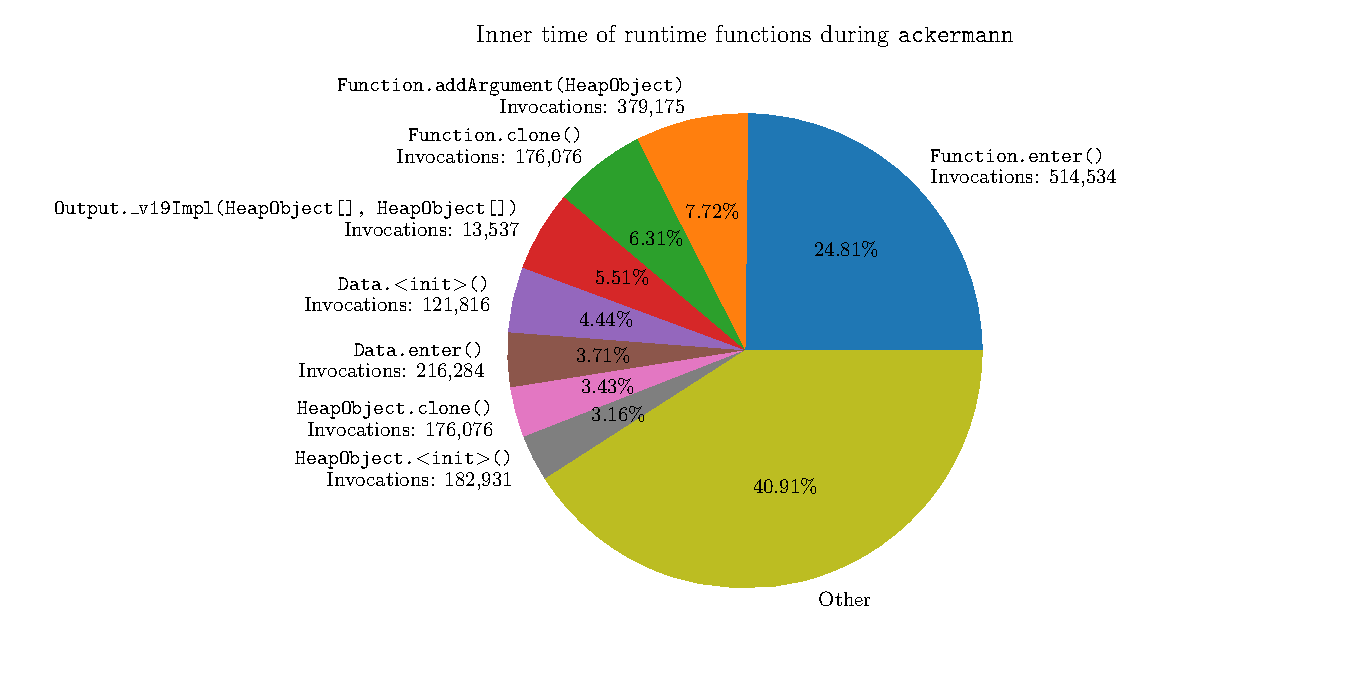
\includegraphics[width=0.7\textwidth]{graphs/perf_profile_ackermann.pdf}
            \caption{A breakdown of the percentage of execution time spent in each Java function in the generated code (`inner time') for the \monospace{ackermann} benchmark. Functions with inner time of less than 3\% are grouped into a single wedge.}
            \label{fig:inner-time}
        \end{figure}

        As described in the implementation chapter, my compiler uses objects of a single class to represent closures, with objects of the class storing \java{Function} objects generated using the \monospace{invokedynamic} instruction and Java 8's support for anonymous functions. This is different from the approaches taken by both Eta and Frege, where closures are translated into anonymous classes that implement a Functional Interface\footnote{\url{https://docs.oracle.com/javase/8/docs/api/java/util/function/package-summary.html}} allowing objects of the classes to be invoked like anonymous methods.

        This design choice was deliberate: before implementing my compiler, it seemed like using a single class for all functions would be more efficient than using a new class for each function, as the equivalent Java code is significantly shorter. After implementation and having compared the two different approaches, using functional interfaces with a new class for each function results in simpler code for the creation and evaluation of closures, which I expect plays a large role in the performance difference.
    }
    \subsection{Compiler Performance}
    {
        Figure \ref{fig:compiler-perf} presents the minimum time taken to compile each benchmark program: my compiler is faster than both Eta and Frege to compile all benchmarks except for \monospace{mergesort}. 

        Figure \ref{fig:compiler-perf-ackermann} shows the same metrics for just the \monospace{ackermann} benchmark on my compiler, so the times for each stage can be seen more clearly. It's clear that code generation is the most expensive stage in the main pipeline: profiling reveals that this is mostly due to the inefficient implementation of parts of the \monospace{hs-java} library. Efforts were made to improve the performance, in one case halving the time spent in code generation\footnote{\url{https://github.com/hnefatl/hs-java/commit/5cbd5c3995161199442310ac30c101b0497a7f98}} for the \monospace{mergesort} benchmark, but as this was an unexpected work package I ran out of time before being able to improve the performance to a satisfactory level.
        
        The poor performance when compiling the \monospace{mergesort} benchmark appears to be due to the large number of bindings involved: processing the list of 1000 input numbers pushes the inefficient stages to their limit. 

        \begin{figure}[h]
            \centering
            \captionsetup{width=0.8\textwidth}
            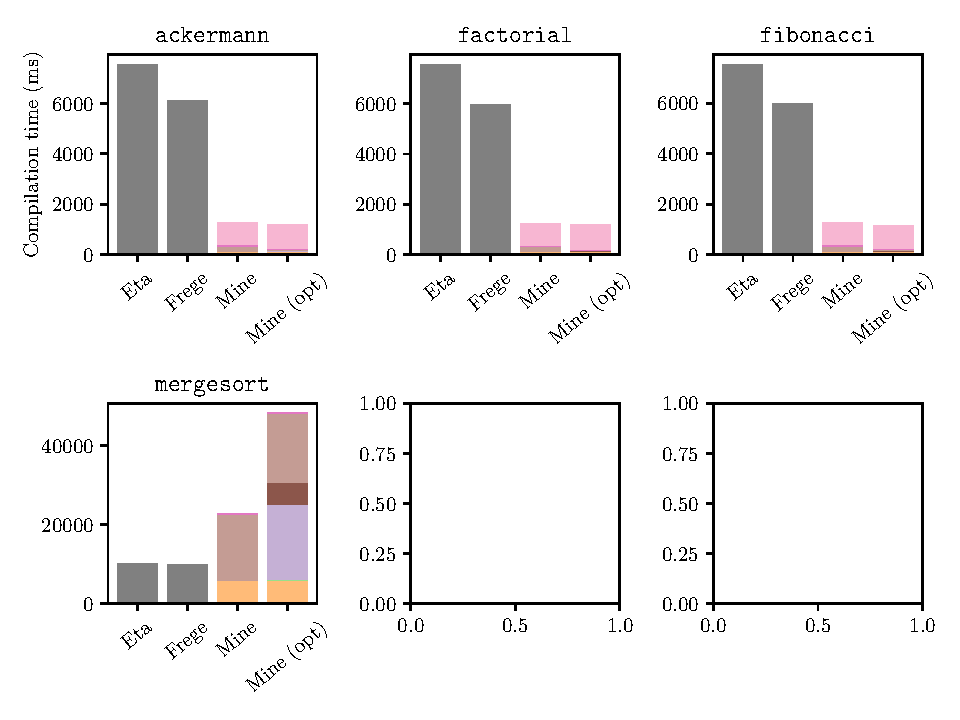
\includegraphics[width=0.9\textwidth]{graphs/compiler_perf.pdf}
            \caption{Minimum time taken to compile the benchmark program. The coloured sections indicate the amount of time spent in each stage of the compiler.}
            \label{fig:compiler-perf}
        \end{figure}
        \begin{figure}[h]
            \centering
            \captionsetup{width=0.8\textwidth}
            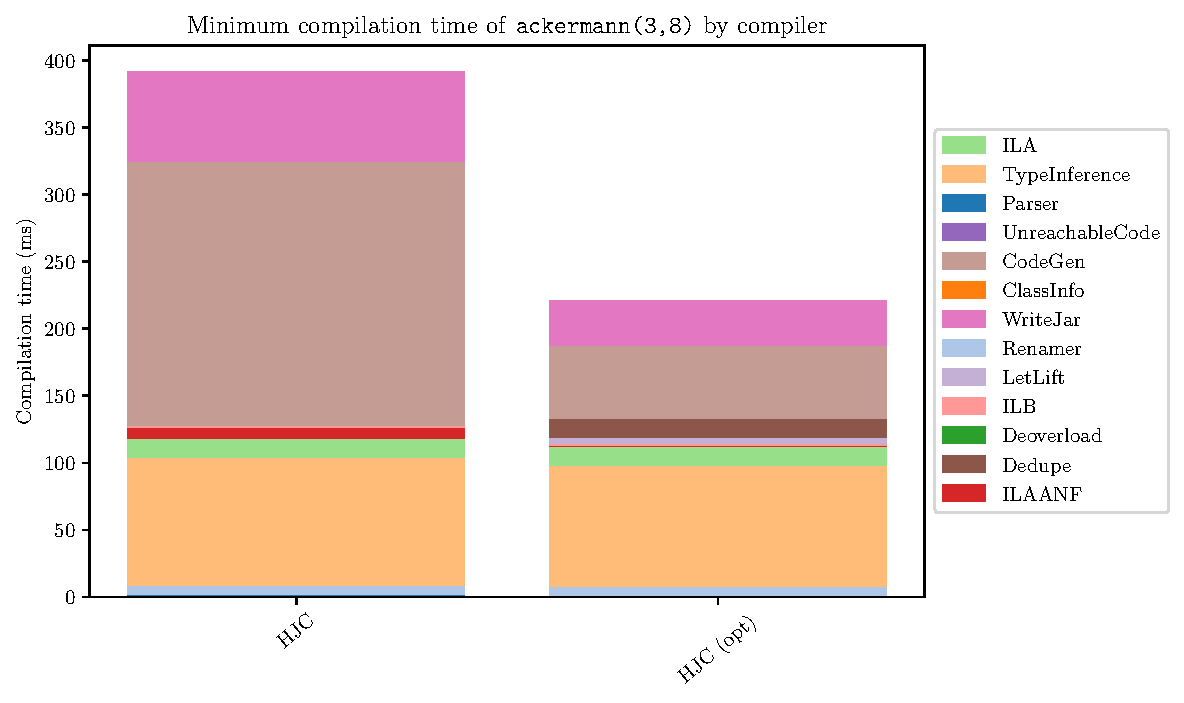
\includegraphics[width=0.9\textwidth]{graphs/compiler_perf_mine_ackermann.pdf}
            \caption{Runtime of each stage in the compiler for the \monospace{ackermann} benchmark.}
            \label{fig:compiler-perf-ackermann}
        \end{figure}

        It's interesting that the compiler usually takes less time to process the input when performing optimisations than when not. This appears to be due to a significant amount of the compilation time being spent in the code generation stage, and compressing and writing the compiled classes into a jar file: the unreachable code elimination optimisation described in Section \ref{sec:unreachable-elim} can massively reduce the amount of code that reaches code generation, which in turn reduces the amount of bytecode that needs to be compressed and written to disk.
    }
    \subsection{Executable Size}
    {
        Figure \ref{fig:executable-size} displays the compiled size of each benchmark program after compilation by the various compilers. All three compilers generate a fixed-size set of class files that implement the logic of the Haskell program, have class files providing runtime support (for example, each compiler has an equivalent to the \java{Function} class described in Section \ref{sec:heap-objects}), and usually have a class file for each datatype defined in the Haskell program. This metric includes specifically the class files implementing the logic from the Haskell code and the runtime files, but does not count the size of the implementation of datatypes or other files. This combination was chosen because all the compilers generate class files for all datatypes regardless of whether they're used by the program, and Frege and Eta implement many more datatypes than my compiler's standard library provides: this causes the size of their executables to be primarily due to datatype implementation, obscuring the size due to the program logic itself.

        Also of note is that Eta and my compiler perform the Java equivalent of static linking, where the executable jar contains both the program logic and all the runtime files required, so that it can execute portably on any machine supporting Java. Frege performs the equivalent of dynamic linking, requiring the compiler's jar to be on the Java classpath when running its output executables as the runtime files are all stored inside. This made accurately measuring executable size slightly trickier.

        \begin{figure}[H]
            \centering
            \captionsetup{width=0.8\textwidth}
            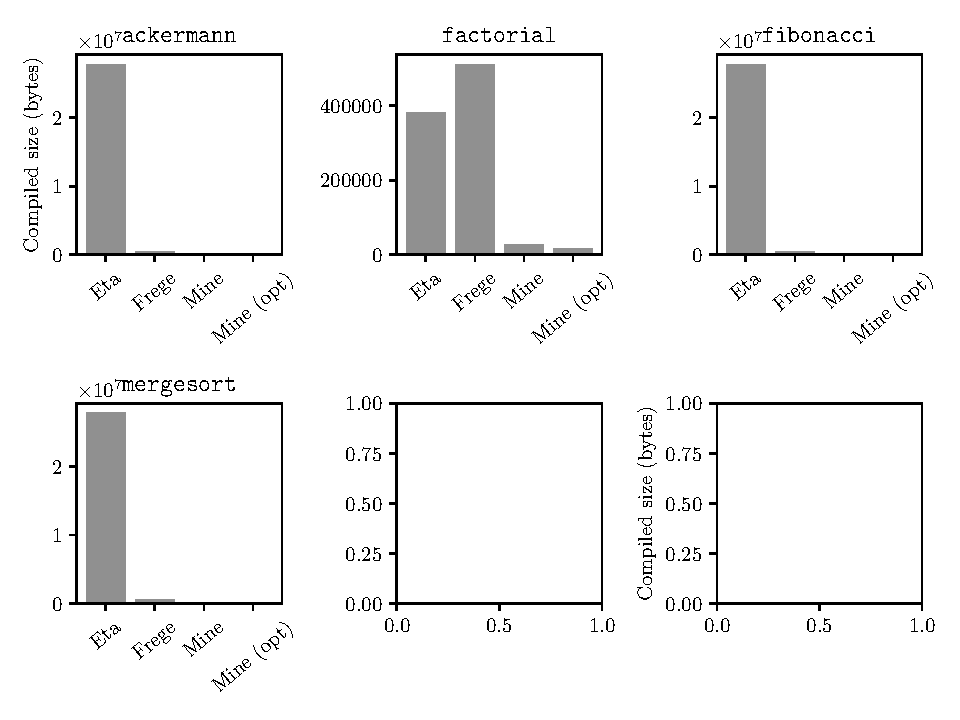
\includegraphics[width=0.9\textwidth]{graphs/size.pdf}
            \caption{Compiled size of each benchmark program. This size includes the runtime system and the bytecode corresponding to the actual program.}
            \label{fig:executable-size}
        \end{figure}
    }
    \subsection{Impact of Optimisations}
    {
        \begin{figure}[H]
            \centering
            \captionsetup{width=0.8\textwidth}
            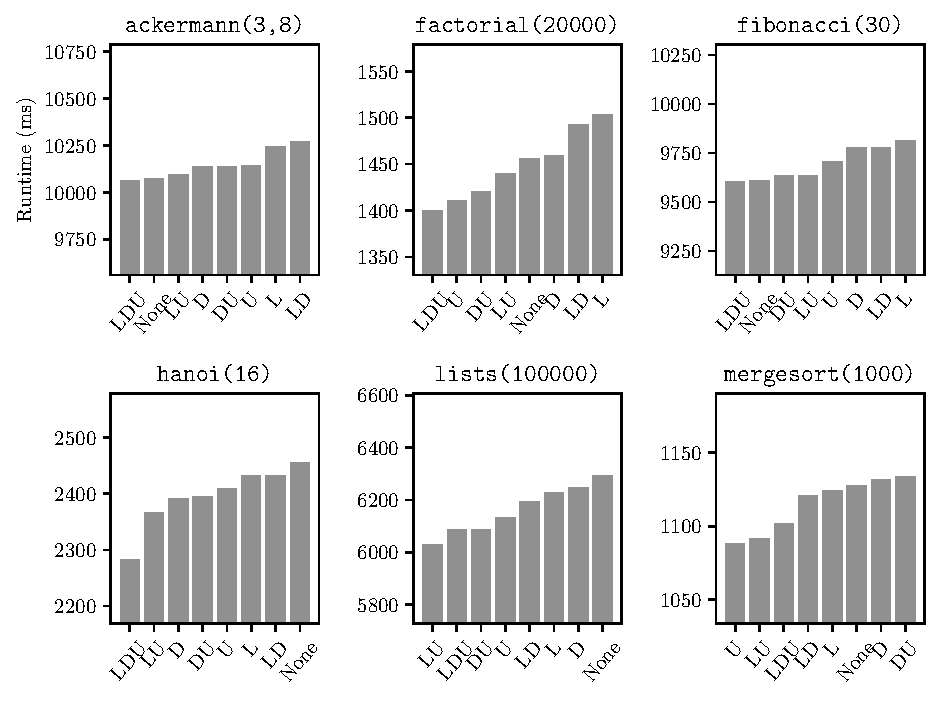
\includegraphics[width=0.9\textwidth]{graphs/perf_by_opt.pdf}
            \caption{Minimum runtime of the benchmarks after compilation with various optimisations: L stands for let-lifting, D for binding deduplication, and U for unreachable code elimination.}
            \label{fig:opt-perf}
        \end{figure}



        \todo[inline]{U produces exactly the same ILB and bytecode for all the functions not eliminated (at least for ackermann). Chalk it up as a mysterious JVM interaction, as the code run is exactly the same. Profiling showed that all functions are called the same number of times!}

        % Write this section. Can excuse U, make some argument about L/D. Want LD to be best speed, so hopefully the new data shows this.

    }
}
\section{Schedule}
{
    \todo[inline]{This is a WIP rehash of the stuff from the progress report explaining why the schedule got messed up, I feel it'll help explain why optimisations didn't get much splotlight.}

    The core features of Haskell are tightly coupled: simple features such as arithmetic operators require a significant level of support for other language features. For example, the \haskell{(+)} function relies on:

    \begin{description}
    \item[Typeclasses:] \haskell{(+)} is defined by the \haskell{Num} typeclass in order to allow ad-hoc overloading.
    \item[Typeclass instances:]
    {
        The types that can be used as arguments to the overloaded functions, and the implementation of the overloads, are defined by typeclass instances.
    }
    \item[Datatypes:]
    {
        The most common implementation of typeclasses involves translating classes into datatypes and instances into values of the datatype.
    }
    \end{description}

    It would be possible to implement a function like \haskell{(+)} which only worked for integers and avoid all of the dependencies on other language features, but then the language simply wouldn't be Haskell: it would resemble a lazy variant of ML's semantics.

    All of these language features are very expensive to implement, as they span multiple layers of the compiler: the type checker needs to be able to infer and check types based on the usage of these features, they need to be translatable into intermediate languages, and the code generator needs to be able to produce bytecode reflecting the semantics. 
}

\end{document}